This section will go through the verification of binary search trees 
and consequently AVL trees in Lean. First I will give some structural definitions for the tree and its properties, 
and then proceed with an explanation of the various proofs completed. 
The textbook released by the University of Pennsylvania \textit{Verified Functional Algorithms} \cite{bst:upenn}
and \textit{Discrete Mathematics with a Computer} \cite{avl:computer} were used as a reference point for some definitions and basic proof statements.

\section{Binary Search Trees}
\subsection*{Binary Search Trees}
The first thing to defining an AVL tree is to define a binary search tree. A binary tree 
definition exists in Lean3 under the inductive type \lstinline{bin_tree}, however the definition is incomplete
for the purpose of binary search. The \lstinline{bin_tree} constructor \lstinline{leaf} is the only one that includes a 
definition for a key, and not the constructor dor \lstinline{node}. We want access to subtrees and the key at any given node 
to define the binary search property, so we create our own definition for a binary tree. This definition can be seen in Figure \ref{lst:btree}.
The type for the structure is inductive, which is useful for proofs as induction can be performed on any \lstinline{btree}.

\begin{figure}[!h]
  \centering
  \lstinputlisting[language=lean, firstline=3, lastline=5, frame=single]{/Users/sofiakonovalova/Desktop/Thesis/lean-thesis/src/basic.lean}
  \caption{}
  \label{lst:btree}
\end{figure}

I also define the basic operations for a binary search tree: \lstinline{insert}, \lstinline{bound},
and \lstinline{lookup}, shown in Figure \ref{lst:basic_ops}. The definition of \lstinline{bound} and \lstinline{lookup} are similar, with bound not serving much reason except for
using it in later proofs to show that node keys are preserved after other operations.  

\begin{figure}[!ht]
  \centering
  \lstinputlisting[language=lean, firstline=12, lastline=31, frame=single]{/Users/sofiakonovalova/Desktop/Thesis/lean-thesis/src/basic.lean}
  \caption{}
  \label{lst:basic_ops}
\end{figure}

I also define the binary search property, as shown in Definition \ref{def:bst_property}. For this I created a helper definition, \lstinline{forall_keys}, which 
defines what exactly it means for all keys in a left or right subtree to be smaller or larger than the root key. This definition is made as abstract as possible, with the 
greater-than or less-than relation defined as just the \notes{parameter? variable? } \lstinline{p}, which is given a type of \lstinline{nat → nat → Prop}, which is the type definition of the 
$>$ and $<$ relations in Lean. If the predicate is satisfied in the current node, as well as the left and right subtrees, then the predicate is satisfied in the whole tree. With this definition,
the formalization of the binary search property is halfway done.

We call the definition for the binary search property \lstinline{ordered}, as
it is another name for trees where the property holds. It is also made recursive, as in our inductive \lstinline{btree} definition, we only have direct definition of the left child and the right child, 
and not the children of those children. There is no guarantee that the grandchildren are ordered, so the definition takes this into account with the recursion: a binary tree can only be ordered if every single subtree 
is ordered. The complete definition can be seen in Figure \ref{lst:ordered}. 

\begin{figure}[!ht]
  \centering
  \lstinputlisting[language=lean, firstline=35, lastline=38, frame=single]{/Users/sofiakonovalova/Desktop/Thesis/lean-thesis/src/basic.lean}
  \caption{}
  \label{lst:forall_keys}
\end{figure}

\begin{figure}[!ht]
  \centering
  \lstinputlisting[language=lean, firstline=40, lastline=43, frame=single]{/Users/sofiakonovalova/Desktop/Thesis/lean-thesis/src/basic.lean}
  \caption{}
  \label{lst:ordered}
\end{figure}

\subsection*{Balancing}
I define the height of a tree as per Definition \ref{def:height} in Figure \ref{lst:height}. \notes{Why is there a +1 in the definition?}

\begin{figure}[!ht]
  \centering
  \lstinputlisting[language=lean, firstline=49, lastline=52, frame=single]{/Users/sofiakonovalova/Desktop/Thesis/lean-thesis/src/basic.lean}
  \caption{}
  \label{lst:height}
\end{figure}

\section{AVL Trees}
I begin by defining a binary search tree. A binary tree is a tree data structure where each node can have no more than two children. These two children are 
called the \textit{left child} and the \textit{right child} subtrees. In a \textit{binary search tree} (BST), nodes are placed according to their key. 

Where nodes are placed in a binary search tree is determined by what is often called the \textit{binary search property}.

\begin{definition}[Binary Search Property]
  \label{def:bst_property}
  Given any node N in a binary search tree, all the keys in the left child subtree are smaller than that of N, and all keys in the right child subtree are greater than the 
  key of N.
\end{definition}

This allows for lookup and insertion to be done in $O \log n$ time in the worst case, as at any given node half of the tree is skipped.

Search, insertion and retrieval can be done recursively. Starting at the root node, the input key and the node key are compared: if the input key is smaller,
the operation is done recursively on the left subtree; if the input key is larger, then the operation is done recursively on the right subtree.

\begin{figure}[!ht]
  \centering
  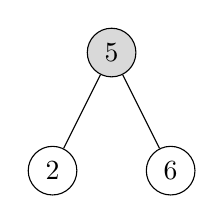
\begin{tikzpicture}
    \node[circle,draw,fill=gray!30](z){5}
        child {
          node[circle,draw]{2}
          child[missing]
          child[missing]
        }
        child{
          node[circle,draw]{6}
          child[missing]
          child[missing]
        };
  \end{tikzpicture}%
  \hspace{1cm}%
      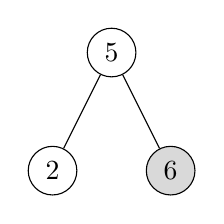
\begin{tikzpicture}
      \node[circle,draw](z){5}
        child {
          node[circle,draw]{2}
          child[missing]
          child[missing]
        }
        child{
          node[circle,draw,fill=gray!30]{6}
          child[missing]
          child[missing]
        };
    \end{tikzpicture}%
    \hspace{1cm}%
    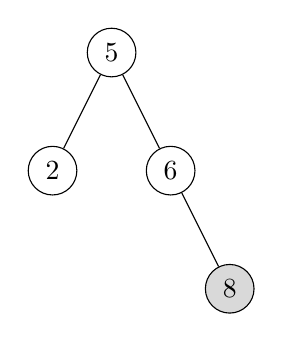
\begin{tikzpicture}
      \node[circle,draw](z){5}
        child {
          node[circle,draw]{2}
          child[missing]
          child[missing]
        }
        child{
          node[circle,draw]{6}
          child[missing]
          child {
            node[circle,draw,fill=gray!30]{8}
            child[missing]
            child[missing]
          }
        };
    \end{tikzpicture}
    \caption{Example of an insertion operation with key 7}
    \label{fig:insert}
\end{figure}

An AVL tree is based on a binary search tree, with one very important distinction - it is \textit{balanced}. To define what it means for a tree to be balanced, I will first
define what the \textit{height} of a tree is.

\begin{definition}[Tree height]
  \label{def:height}
  The height of a tree is the length of the longest path from the root to a leaf.
\end{definition} 
 
Balance is reliant on this definition - an AVL tree is only balanced when the 
heights of any given left and right child subtrees does not differ by more than one \cite{avl:original}. By keeping balance, the structure ensures that there is a high ratio between the number of 
nodes in the tree and the height. This allows for retrieval and search operations to be done in $O(\log n)$ time in the worst case, with $n$ being the amount of nodes in a tree \cite{avl:computer}. A
balancing factor can help define whether a tree is balanced or not.

\begin{definition}[Balancing factor]
  \label{def:bf}
  The balancing factor $BF(n)$ of a tree is the difference in height between the left child tree and the right child tree. A tree is defined to be an AVL tree (and therefore balanced) is the
  invariant $BF(n) \in \{-1,0,1\}$ holds for every node $n$ in the tree.
\end{definition}

During node insertion, the tree can become imbalanced, which can be mitigated
with either a right rotation or a left rotation. 

\begin{figure}[!ht]
  \centering
  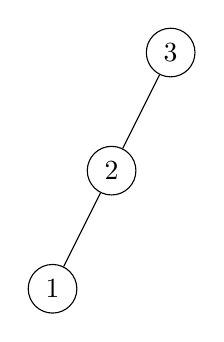
\begin{tikzpicture}
    \node[circle,draw](z){3}
      child {
        node[circle,draw]{2}
        child {
          node[circle,draw]{1}
          child[missing]
          child[missing]
        }
        child[missing]
      }
      child[missing];
  \end{tikzpicture}%
  \hspace{1cm}%
  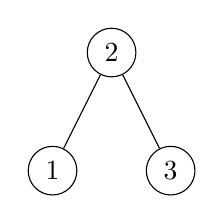
\begin{tikzpicture}
    \node[circle,draw](z){2}
    child{
      node[circle,draw]{1}
      child[missing]
      child[missing]
    }
    child{
      node[circle,draw]{3}
      child[missing]
      child[missing]
    };
  \end{tikzpicture}
  \caption{Example of a single right rotation}
  \label{fig:right_rotation}
\end{figure}

\section{Proofs}
In this section, we verify the operations presented above. Each subsection details examples of proof statements for specific operations and informally explains how to complete the proofs. AVL tree operations need to restore balance, as well as preserve order and keys. This section does not detail all of the proof constructions, but goes give all the necessary lemmas and proofs are detailed when it is either important to understand the proof statement or when the proof construction led to core design decisions. The lemma statements presented here closely follow \cite{textbook:discrete_computer}, though some changes were made to statements to suit the Lean definitions.

\subsection{BST Operations}
First, we prove two lemmas related to boundedness and lookup in a tree, since \lstinline{lookup} and \lstinline{bound} are identical for both BSTs and AVL trees.

\begin{lstlisting}
lemma bound_false (k : nat) (t : btree α) :
  bound k t = ff → lookup k t = none := ...

lemma bound_lookup (k : nat) (t : btree α) :
  ordered t → bound k t → ∃ (v : α), lookup k t = some v := ...
\end{lstlisting}

The lemma \lstinline{bound_false} states that if a key is not bound in a tree, then lookup will not result in any node data being returned. The lemma \lstinline{bound_lookup} states that if a key is bound in a tree, then some data will be returned. The existential quantifier is used in this lemma, because we cannot make assumptions on which key will return which value. In other words, we don't know the specific node value, but we do know that something will be returned. Both of the proofs were constructed by induction on the tree \lstinline{t}.

\subsection{Rotation}
With rotations we want to prove that an ordered tree preserves order after a rotation, and that if a tree is imbalanced then a rotation restores its balance. This section will present two proofs on right rotations preserving order and balance.

\subsection*{Order}
\begin{lstlisting}[caption=\empty, label={lst:right_ordered}]
lemma rotate_right_ordered (t : btree α) :
  ordered t → ordered (rotate_right t) := ...
\end{lstlisting}

Listing \ref{lst:right_ordered} shows a formalized lemma statement for right rotations preserving order. The first step with proof statements with rotations is to look at their definitions. The definition for \lstinline{rotate_right} uses the \lstinline{simple_right} and \lstinline{simple_left} definitions, so proofs about them preserving order need to be constructed too.

\begin{lstlisting}[caption=\empty, label={lst:simple_ordered}]
lemma simple_right_ordered (t : btree α) :
  ordered t → ordered (simple_right t) := ...

lemma simple_left_ordered (t : btree α) :
  ordered t → ordered (simple_left t) := ...
\end{lstlisting}

The proof in Listing \ref{lst:right_ordered} were done by case splitting on the tree \lstinline{t}, its right subtree \lstinline{r} and the next subtree \lstinline{lr}, and the simple rotation lemmas were applied throughout when needed. The simple rotation lemmas were also completed by case splitting on left or right subtree depending on the rotation.

The proofs above also require a lemma for transitivity of keys in trees. Assume a tree \lstinline{rr} and \lstinline{rl}, with the former having a left and a right child \lstinline{rll} and \lstinline{rlr}. Also assume two keys \lstinline{rk}, which is the parent node key of \lstinline{rr}, and \lstinline{rlk}, which is the key of \lstinline{rl}.
If \lstinline{rk} is greater than all the keys contained in \lstinline{rll} and \lstinline{rlr}, and \lstinline{rk} is less than the keys in \lstinline{rr}, by transitivity \lstinline{rlk} is less than all the keys in \lstinline{rr}. The lemma for key transitivity is formalized below.

\begin{lstlisting}[caption=\empty]
lemma forall_keys_trans (t : btree α) (p : nat → nat → Prop) 
(z x : nat) (h₁ : p x z) (h₂ : ∀ a b c, p a b → p b c → p a c) :
  forall_keys p z t → forall_keys p x t := ...
\end{lstlisting}

Another lemma had to be made to make constructing proofs with \lstinline{forall_keys} much easier. The current definition for \lstinline{forall_keys} does not take into consideration the relationship of the input key between the left and right children of the tree. The \lstinline{forall_keys_intro} introduction lemma solved this problem.

\begin{lstlisting}[caption=\empty]
lemma forall_keys_intro {l r : btree α} {k x : nat} {v : α} 
  {p : nat → nat → Prop} :
(forall_keys p k l ∧ p k x ∧ forall_keys p k r) 
  → forall_keys p k (node l x v r) := ...
\end{lstlisting}

When applying the introduction lemma, I was able to get the relation of the key between the left and right subtree, and the relation between the input key and the key of the tree, which made applying the transitivity lemma a lot easier.

\subsection*{Balance}

\subsection{Insertion}
Proofs about insertion into AVL trees, like the ones for rotation, need to show a preservation of order, keys, and balance restoration.

\subsection{Deletion}
This section will go through the proof construction of deletion preserving order, and the sub-proofs that come along with it as well as major changes that have been done to previous definitions to make the proof constructions easier and readable.

The lemma statement for deletion preserving order is formalized below.

\begin{lstlisting}[caption=\empty]
lemma delete_ordered (t : btree α) (k : nat) :
  ordered t → ordered (delete k t) :=
\end{lstlisting}

Since the function \lstinline{delete} uses \lstinline{del_node}, a similar proof has to be constructed for it as well. The lemma statement does not contain a key, as with \lstinline{del_node}, the tree is assumed to have the root that matches the key in the arguments of \lstinline{delete}.

\begin{lstlisting}[caption=\empty]
lemma del_node_ordered (t : btree α) (k : nat) :
  ordered t → ordered (del_node t) :=
\end{lstlisting}

Both of the above proofs were constructed by induction on the tree \lstinline{t}.

Since \lstinline{del_node} uses \lstinline{shrink}, a proof for \lstinline{shrink} preserving order needs to be constructed as well. The lemma statement needs to have the reuslt of \lstinline{shrink} as one of its hypotheses, and the conclusion is that the result of shrinking a tree is also ordered, and that the resulting key is larger than the keys in the shrunken tree.

\begin{lstlisting}[caption=\empty, label={lst:shrink_ordered}]
lemma shrink_ordered {t sh : btree α} {x : nat} {a : α} :
  ordered t ∧ shrink t = some (x, a, sh) → ordered sh ∧ forall_keys gt x sh :=
\end{lstlisting}

The proof for \lstinline{shrink_ordered} was done by induction on the tree, but generalizing \lstinline{x}, \lstinline{a} and \lstinline{sh}. This is because without the generalization, the proof would be referring to a specific result of \lstinline{shrink}, which cannot be foreseen, so therefore the proof needs to take into account all the possible values for the three-tuple result of \lstinline{shrink}.

During the proof, I came across a sitation where some of the hypotheses were about \lstinline{shrink}, but no information could be derived from them. This led to the creation of a view\footnote{\notes{write how this was done by the supervisor but idk how yet}} for \lstinline{shrink}, to show each possible variation of arguments for \lstinline{shrink} and the result that gives.

\begin{lstlisting}[caption=\empty]
inductive shrink_view {α} : btree α → option (nat × α × btree α) → Sort*
| empty : shrink_view empty none
| nonempty_empty : ∀ {l k v r},
  shrink r = none →
  shrink_view (node l k v r) (some (k, v, l))
| nonempty_nonempty₁ : ∀ {l k v r x a sh out},
  shrink r = some (x, a, sh) →
  height l > height sh + 1 →
  out = some (x, a, rotate_right (btree.node l k v sh)) →
  shrink_view (node l k v r) out
| nonempty_nonempty₂ : ∀ {l k v r x a sh},
  shrink r = some (x, a, sh) →
  height l ≤ height sh + 1 →
  shrink_view (node l k v r) (some (x, a, node l k v sh))
\end{lstlisting}

A lemma was also written for \lstinline{shrink_view}, that would result in case splits for each case in the view. 

\begin{lstlisting}[caption=\empty, label={lst:shrink_view}]
lemma shrink_shrink_view (t : btree α) : 
  shrink_view t (shrink t) :=
\end{lstlisting}

Applying the lemma shown in Listing \ref{lst:shrink_view} would result in three cases in the inductive step of the proof in Listing \ref{lst:shrink_ordered}.